\input{header}
\usetheme{antibes}
\title{Torsion subgroups of elliptic curves in Lean}
\subtitle{SMS Spring Meeting: Formalization and Proof Assistants}
\author{David Kurniadi Angdinata (with Chris Birkbeck)}
\institute{University of East Anglia}
\date{Thursday, 26 March 2026}

\begin{document}

\frame\maketitle

\begin{frame}{Elliptic curves}

Elliptic curves are algebraic curves given by cubic equations, whose set of points can be endowed with the structure of an abelian group.

\bigskip

\begin{minipage}{0.4\textwidth}
\begin{center}
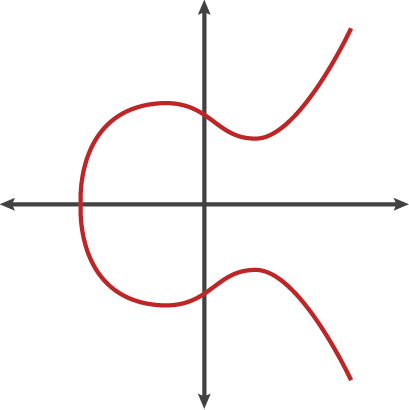
\includegraphics[width=\textwidth]{img/ellipticcurve.png}
\end{center}
\end{minipage}
\begin{minipage}{0.59\textwidth}
\begin{itemize}
\item Wiles's proof of Fermat's last theorem is a correspondence between elliptic curves and certain modular forms.
\item The Birch and Swinnerton-Dyer conjecture predicts the rank of an elliptic curves in terms of L-functions.
\item Intractability of the discrete logarithm problem forms the basis behind many public key cryptographic protocols.
\item The Atkin--Morain primality test and Lenstra's factorisation method are two of the fastest known algorithms.
\end{itemize}
\end{minipage}

\end{frame}

\begin{frame}{Weierstrass equations}

Formally, an \textbf{elliptic curve $ E $ over a field $ F $} is a smooth projective curve of genus one over $ F $ with a distinguished point $ O $ defined over $ F $.

\bigskip By the Riemann--Roch theorem, its set of points $ E(F) $ is the zero locus of
$$ f := Y^2 + a_1XY + a_3Y - (X^3 + a_2X^2 + a_4X + a_6), $$
for some $ a_i \in F $ such that $ \Delta \ne 0 $, \footnote{\tiny $ \Delta := -(a_1^2 + 4a_2)^2(a_1^2a_6 + 4a_2a_6 - a_1a_3a_4 + a_2a_3^2 - a_4^2) - 8(2a_4 + a_1a_3)^3 - 27(a_3^2 + 4a_6)^2 + 9(a_1^2 + 4a_2)(2a_4 + a_1a_3)(a_3^2 + 4a_6) $} with $ O $ being the point at infinity.

\bigskip More specifically, there is an equivalence of categories
$$ \{\text{elliptic curves over} \ F\} \cong \{(a_1, a_2, a_3, a_4, a_6) \in F^5 \ \text{such that} \ \Delta \ne 0\}. $$
In \texttt{mathlib}, an \textbf{elliptic curve $ E $ over a ring $ R $} is the data of a tuple $ (a_1, a_2, a_3, a_4, a_6) \in R^5 $ and a proof that $ \Delta \in R^\times $. A \textbf{point} in $ E(F) $ is either $ O $ or an \textbf{affine point} $ (x, y) \in R^2 $ such that $ f(x, y) = 0 $.

\end{frame}

\begin{frame}{Group law}

There is an \textbf{addition law} of points in $ E(F) $ defined geometrically.

\begin{center}
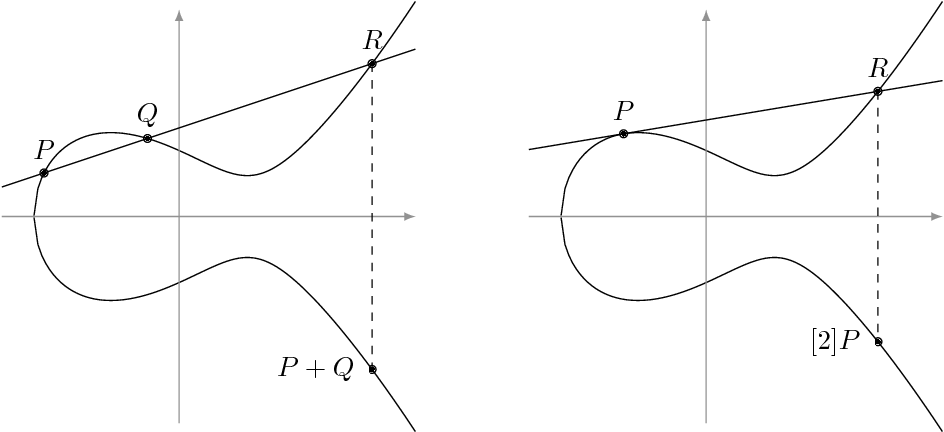
\includegraphics[width=0.8\textwidth]{img/grouplaw.png}
\end{center}

In \texttt{mathlib}, the addition law is given by explicit rational functions.

\begin{formalisation}[A.--Xu, 2022]
This addition law makes $ E(F) $ an abelian group with identity $ O $.
\end{formalisation}

\end{frame}

\begin{frame}{The $ n $-torsion subgroup}

For any $ P \in E(F) $ and any $ n \in \Z $, denote multiplication-by-$ n $ by
$$ [n](P) := \underbrace{P + \dots + P}_n, $$
and define the \textbf{$ n $-torsion subgroup} by $ E(F)[n] := \ker[n] $.

\begin{formalisation}[A.--Xu, 2024]
If the characteristic of $ F $ does not divide $ n $, then $ \#E(\overline{F})[n] = n^2 $.
\end{formalisation}

\begin{exercise}[3.7(d) in \emph{The Arithmetic of Elliptic Curves} by Silverman]
Prove that for any affine point $ (x, y) \in E(F) $,
$$ [n](x, y) = \left(\dfrac{\phi_n(x, y)}{\psi_n(x, y)^2}, \dfrac{\omega_n(x, y)}{\psi_n(x, y)^3}\right). $$
\end{exercise}

\end{frame}

\begin{frame}{Division polynomials}

Assume $ a_1 = a_2 = a_3 = 0 $. Then $ \phi_n, \omega_n, \psi_n \in F[X, Y] $ are defined by

{\footnotesize
\begin{minipage}{0.5\textwidth}
\begin{align*}
\psi_0 & := 0, \\
\psi_1 & := 1, \\
\psi_2 & := 2Y, \\
\psi_3 & := 3X^4 + 6a_4X^2 + 12a_6X - a_4^2, \\
\psi_4 & := \psi_2 \cdot (2X^6 + 10a_4X^4 + 40a_6X^3 \\
& \qquad - 10a_4^2X^2 - 8a_4a_6X - 4a_6^2 - 2a_4^3),
\end{align*}
\end{minipage}
\begin{minipage}{0.49\textwidth}
\begin{align*}
\psi_{2n + 1} & := \psi_{n + 2}\psi_n^3 - \psi_{n - 1}\psi_{n + 1}^3, \\
\psi_{2n} & := \dfrac{\psi_{n - 1}^2\psi_n\psi_{n + 2} - \psi_{n - 2}\psi_n\psi_{n + 1}^2}{\psi_2}, \\
\psi_{-n} & := -\psi_n, \\
\phi_n & := X\psi_n^2 - \psi_{n + 1}\psi_{n - 1}, \\
\omega_n & := \dfrac{\psi_{2n}}{2\psi_n}.
\end{align*}
\end{minipage}
}

\bigskip Observe that $ \phi_n $ and $ \psi_n^2 $ can be viewed as polynomials in $ F[X] $ modulo $ f $.

\begin{exercise}[3.7(b) in \emph{The Arithmetic of Elliptic Curves} by Silverman]
Prove that $ \phi_n = X^{n^2} + \dots $ and $ \psi_n^2 = n^2X^{n^2 - 1} + \dots $.
\end{exercise}

\end{frame}

\begin{frame}{Arithmetic structure}

\begin{theorem}[Mordell--Weil, 1929]
If $ K $ is a global field, then $ E(K) $ is finitely generated.
\end{theorem}

By the structure theorem for finitely generated abelian groups,
$$ E(K) \cong \tor(E / K) \oplus \Z^{\rk(E / K)}, $$
where $ \rk(E / K) \in \N $ is the \textbf{rank}, and the finite \textbf{torsion subgroup} is
$$ \tor(E / K) := \bigcup_{n \in \Z \setminus \{0\}} E(K)[n] \le E(K). $$
The proof of Mordell--Weil has two parts:
\begin{itemize}
\item Weak Mordell--Weil: $ E(K) / nE(K) $ is finite for any $ n \in \Z \setminus \{0\} $.
\item Heights and descent: there is a height function on $ E(K) $.
\end{itemize}
Michael Stoll formalised the latter a month ago.

\end{frame}

\begin{frame}{The torsion subgroup}

While $ \rk(E / K) $ is mysterious, $ \tor(E / K) $ is well-understood.

\begin{theorem}[Levin, 1968]
If $ K $ is the function field of a curve of genus $ g $ over a finite field, then $ \#\tor(E / K) $ is bounded in terms of $ g $.
\end{theorem}

\begin{theorem}[Merel, 1996]
If $ K $ is a number field, then $ \#\tor(E / K) $ is bounded in terms of $ [K : \Q] $.
\end{theorem}

\begin{theorem}[Mazur, 1978]
$$ \tor(E / \Q) \cong
\begin{cases}
C_n, & \text{for} \ n = 1, \dots, 10, 12, \\
C_2 \oplus C_{2n}, & \text{for} \ n = 1, \dots, 4.
\end{cases}
$$
\end{theorem}

\end{frame}

\begin{frame}{Computing torsion subgroups}

\begin{theorem}[Lutz--Nagell, 1937]
Let $ E $ be an elliptic curve over $ \Q $ with $ a_1 = a_2 = a_3 = 0 $ and $ a_4, a_6 \in \Z $. If $ (x, y) \in \tor(E / \Q) $, then
\begin{enumerate}
\item $ x, y \in \Z $, and
\item either $ y = 0 $ or $ y^2 \mid 4a_4^3 + 27a_6^2 $.
\end{enumerate}
\end{theorem}

Note that $ \Delta = -16(4a_4^3 + 27a_6^2) $, and
$$ 4a_4^3 + 27a_6^2 = 3(3y^2 + 4a_4x + 6a_6)y^2 - (3x^2 + 4a_4)\psi_3(x, y). $$
To compute $ \tor(E / \Q) $:
\begin{itemize}
\item Find all $ y \in \Z $ such that $ y^2 \mid 4a_4^3 + 27a_6^2 $.
\item For each such $ y $, find all $ x \in \Z $ such that $ x^3 + a_4x + (a_6 - y^2) = 0 $.
\item For each such $ (x, y) $, check that it is in $ \tor(E / \Q) $.
\end{itemize}

\end{frame}

\begin{frame}{An illustrative example}

Let $ E $ be the elliptic curve $ y^2 = x^3 + 8 $ over $ \Q $ and $ (x, y) \in \tor(E / \Q) $. Then $ x, y \in \Z $, and either $ y = 0 $ or $ y^2 \mid 1728 = 2^6 \cdot 3^3 $. Hence,
\begin{align*}
y^2
& \in \{0, 1, 2, 3, 4, 6, 8, 9, 12, 16, 18, 24, 27, 32, 36, 48, 54, 64, \\
& \qquad 72, 96, 108, 144, 192, 216, 288, 432, 576, 864, 1728\}.
\end{align*}
$$
\begin{array}{|c|c|c|c|c|c|c|c|c|c|}
\hline
y^2 & 0 & 1 & 4 & 9 & 16 & 36 & 64 & 144 & 576 \\
\hline
8 - y^2 & 8 & 7 & 4 & -1 & -8 & -28 & -56 & -136 & -568 \\
\hline
x & -2 & \text{N/A} & \text{N/A} & 1 & 2 & \text{N/A} & \text{N/A} & \text{N/A} & \text{N/A} \\
\hline
y & 0 & \pm1 & \pm2 & \pm3 & \pm4 & \pm6 & \pm8 & \pm12 & \pm24 \\
\hline
\end{array}
$$
Therefore, $ (x, y) \in \{(-2, 0), (1, \pm3), (2, \pm4)\} $. Now,
$$ [2](-2, 0) = O, \quad [2](1, \pm3) = (-\tfrac{7}{4}, \mp\tfrac{13}{8}), \quad [2](2, \pm4) = (-\tfrac{7}{4}, \pm\tfrac{13}{8}). $$
Thus, $ \tor(E / \Q) = \{O, (-2, 0)\} $. In fact, $ \tor(E / \Q) = \langle(-2, 0)\rangle \cong C_2 $.

\end{frame}

\begin{frame}{An elementary proof}

Let $ (x, y) \in \tor(E / \Q) $ such that $ y^2 = x^3 + a_4x + a_6 $. May write
$$ x = \dfrac{b}{d^2}, \qquad y = \dfrac{c}{d^3}, \qquad (b, d) = (c, d) = 1. $$
If $ [n](x, y) \in \Z^2 $, then $ (x, y) \in \Z^2 $, since the $ X $-coordinate of $ [n](x, y) $ is
$$ \dfrac{\phi_n(x, y)}{\psi_n(x, y)^2} = \dfrac{x^{n^2} + \dots}{n^2x^{n^2 - 1} + \dots} = \dfrac{b^{n^2} + d^2(\dots)}{d^2(n^2b^{n^2 - 1} + \dots)}. $$
May assume that $ [p](x, y) = O $ for $ p > 2 $. Then $ \psi_p(x, y) = 0 $, so
$$ 0 = \psi_p(x, y)^2 = p^2x^{p^2 - 1} + \dots = \dfrac{p^2b^{p^2 - 1} + d^2(\dots)}{d^{2(p^2 - 1)}}. $$
Thus $ (x, y) \in \Z^2 $. Now the $ X $-coordinate of $ [2](x, y) \in \tor(E / \Q) $ is $ x - \psi_3(x, y) / 4y^2 $, so $ y^2 \mid \psi_3(x, y) $, and hence $ y^2 \mid 4a_4^3 + 27a_6^2 $.

\end{frame}

\begin{frame}{Lean formalisation}

Chris, ChatGPT, and Claude Code (CCCC) formalised this in a day!

\begin{theorem}[CCCC, 2026]
Let $ E $ be an elliptic curve over a number field $ K $ of class number one with $ a_1 = a_3 = 0 $ and $ a_2, a_4, a_6 \in \OO_K $. If $ (x, y) \in \tor(E / K) $, and the primes dividing the order of $ (x, y) $ do not ramify in $ K $, then
\begin{itemize}
\item $ x, y \in \OO_K $, and
\item either $ y = 0 $ or $ y^2 \mid (4a_4^3 + 27a_6^2) + a_2(4a_2^2a_6 - a_2a_4^2 - 18a_4a_6) $.
\end{itemize}
\end{theorem}

When $ a_1 \ne 0 $ or $ a_3 \ne 0 $, they proved an alternative statement with $ y^2 \mid \Delta $.

\bigskip I am automating the computations of $ \tor(E / \Q) $ using \texttt{simproc}s.

\bigskip When $ 4a_4^3 + 27a_6^2 $ is massive, its factorisation can be extracted from the LMFDB to circumvent divisor \texttt{dsimproc}s, which uses trial division.

\end{frame}

\end{document}